The ultimate goal is to drive the robot into the target position. The target position is in the point ($x_{ref}$,$y_{ref}$). For that we need to define a new variable $\Delta d$. $\Delta d$ is the distance between the current location of the robot ($x$,$y$) and the target location ($x_{ref}$,$y_{ref}$). $\Delta d$ is calculated as follws
\begin{equation} \label{eq89}
\Delta d 
=\sqrt{(x_{ref}-x)^2+(y_{ref}-y)^2}
\end{equation}

In order to arrive to the target location the $\Delta d$ must go to zero. 
We will define a point D in space. The point D is choosen as the point what lies on the robot orientational axis and is the closest point to the target location. Next we will define the angle $\beta$.
$\beta$ is the angle between the line from the robot to the target point and the x axis. Additionally we can define that $\Delta S$ is the distance from the robot to the point D. Those variables are written mathematically as follows:
\begin{equation} \label{eq90}
\beta=atan(y_{ref}-y,x_{ref}-x)
\end{equation}

\begin{equation} \label{eq91}
e_{\theta}=\beta-\theta
\end{equation}

\begin{equation} \label{eq92}
\delta s= \Delta d cos(e_{\theta})
\end{equation}

The control of the system must be done so that the $\Delta s$ and $e_{\theta}$ goes to zero. If both of them are zero then we can presume that the robot have arrived in the target location.
We can now notice that if we are at the point D then the $S_{ref}$-$S$=$\Delta s$. And we can now see that
\begin{equation} \label{eq93}
e_{s}=\Delta s
\end{equation}

We can define the control law as
\begin{equation} \label{eq94}
v=k_{s}e_{s}
\end{equation}

\begin{equation} \label{eq95}
\omega=k_{\theta}e_{\theta}
\end{equation}

In figure \ref{fig:wholesystem} we can see that the part from the error calculations til the kinematics is  linear. Only the error calculation and the kinimatics blocks are non linear. Since there are non linear parts in our model we must conclude that all of the closed loop system is nonlinear.


\begin{figure} 
\centering
 	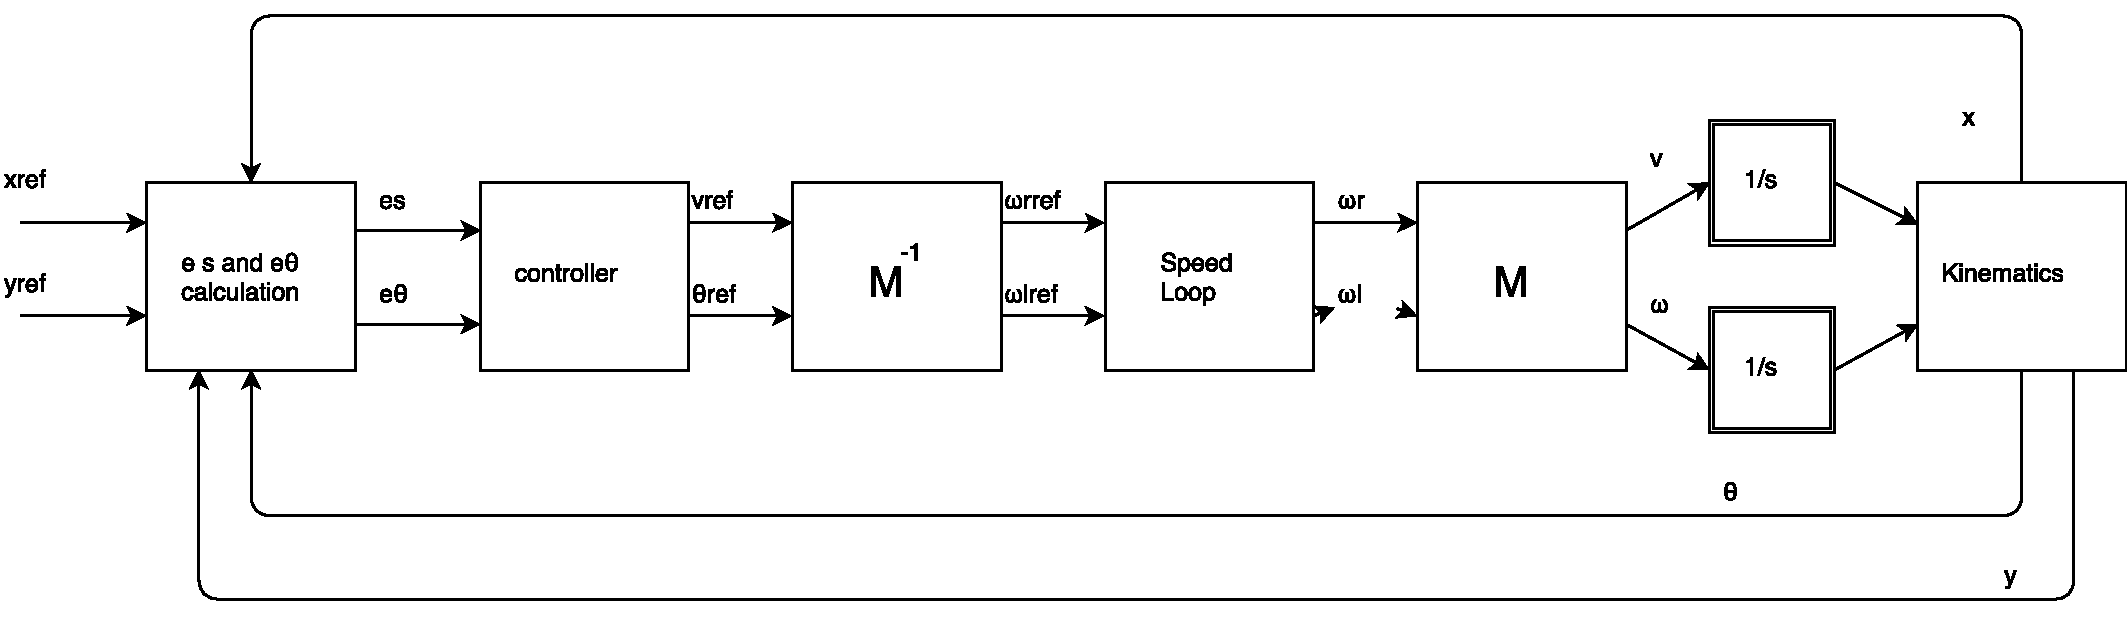
\includegraphics[width=1\textwidth]{figures/cartWxy.pdf}
	
	
	\caption{Whole system block diagram} 
 	\label{fig:wholesystem} 
\end{figure}

When we examin the equations \ref{eq90} and \ref{eq91} we can see that if the point ($x$,$y$) goes to ($x_{ref}$,$y_{ref}$) the control law becomes undifined. In order to avoid this situation we can rewrite the control law as:
\begin{equation} \label{eq96}
v=k_{s} \sqrt{(x_{ref}-x)^2+(y_{ref}-y)^2}
\end{equation}
\begin{equation} \label{eq97}
\omega = 0
\end{equation}

In this form the control law will not become undefined if we are approaching towards the target point.